\section{Simulation and Numerical Results}
\label{sec:result}
For quantum simulation, we used QuTiP5 \cite{qutip5} software.
We first see the results from $X$ gate simulation.
\subsection{X gate}
Simulation has been conducted with the Hamiltonian in \eref{eq:Hrwa} with $N_{max}=3$.
Among several solvers that QuTiP provides, the Shroedinger solver has been chosen.
This is enough unless your target fidelity level is exceedingly low so that the effect of decoherence is visible in the
duration of one gate operation.
The parameters we use for this simulation are
\begin{itemize}
  \item $\Delta/2\pi = -0.225~\text{GHz}$ (anharmonicity),
  \item $\lambda_k = \sqrt{k}$.
\end{itemize}
We set the time slice number of the ODE solver as $25000$. (Increasing this number didn't change the simulation results.)
% We chose the proportionality constant of $\lambda_{k,k+3}$ as $c=0.004$ , we set
% $\lambda_k = \sqrt{k}$, $\lambda_{k,k+3}=c\sqrt{k+1}\sqrt{k+2}\sqrt{k+3}$, with .
% The $X$ gate was implemented with different pulse shapes.
\subsubsection{Fidelity}
The gate infidelity was computed as $\mathcal{E}(\hat{U}_Q) = 1 -
  \mathcal{F}[\hat{U}_Q]$ where $\mathcal{F}[\hat{U}_Q]$ is the gate fidelity defined as
\cite{fidelity}
\begin{equation}
  \label{eq:fidelity}
  \mathcal{F}[\hat{U}_Q] = \frac{\text{Tr}[\hat{U}_Q\hat{U}_Q^\dagger]}{d(d+1)} +
  \frac{\left\vert{}\text{Tr}[\hat{U}_Q\hat{U}_I^\dagger]\right\vert{}^2}{d(d+1)}.
\end{equation}

\begin{figure}[htpb]
  \centering
  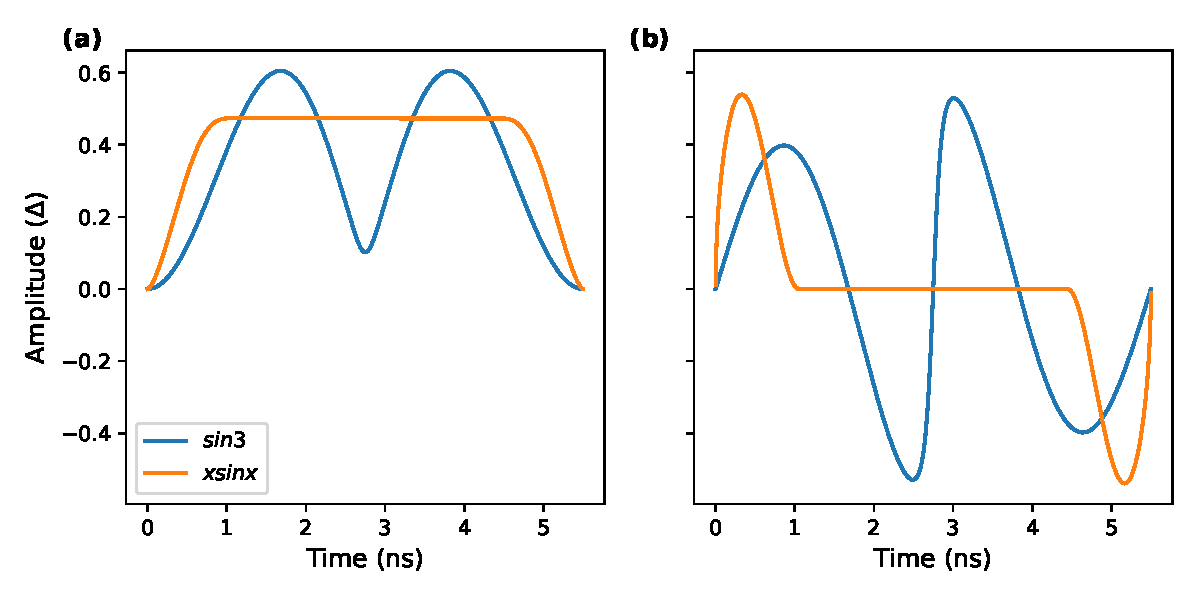
\includegraphics[width=0.8\columnwidth]{fig/fig_r1d_comparison.pdf}
  \label{fig:r1d_comparison}
  \caption{Comparison of $X$ and $Y$ controls of our DRAG-1 (orange) and R1D (blue) pulses.
    (a) $X$ control, (b) $Y$ control.
  }
\end{figure}


\begin{figure}[htpb]
  \centering
  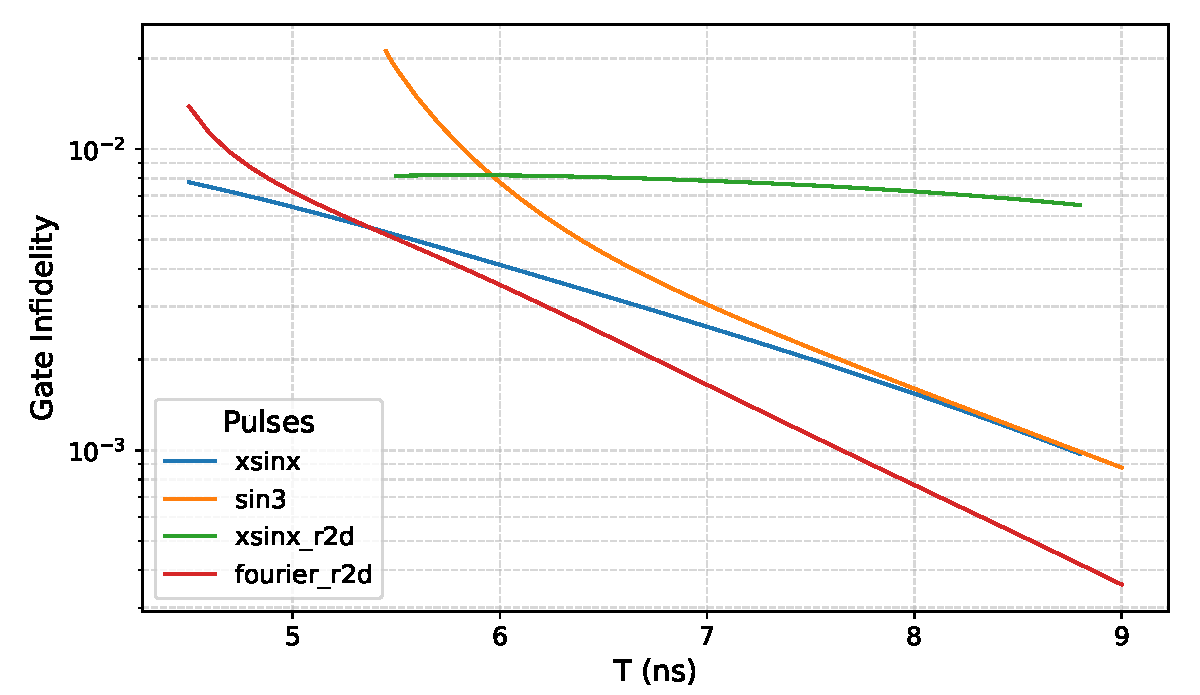
\includegraphics[width=0.8\columnwidth]{fig/fig_gateinfidelity.pdf}
  \label{fig:gate_infidelity}
  \caption{Although our DRAG-2 pulse shows poor performance,
    our DRAG-1 pulse surpasses the performance of the R2D pulse for $T< 5.3~\text{ns}$.}
\end{figure}

\begin{figure}[htpb]
  \centering
  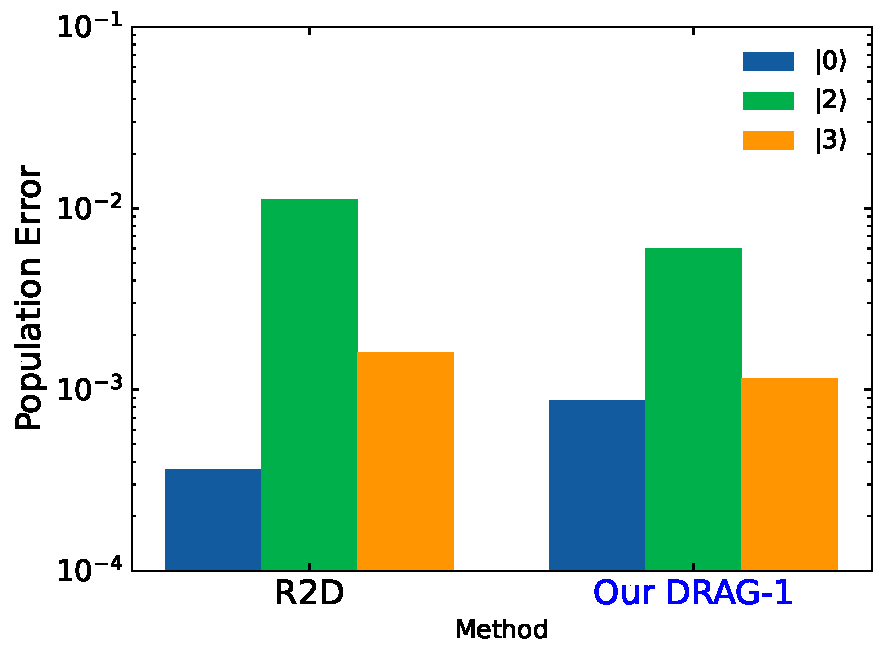
\includegraphics[width=0.8\columnwidth]{fig/fig1d.pdf}
  \label{fig:r2dvsxsinx}
  \caption{Population distirbution of $X$ gate for $T=4.8~\text{ns}$ implemented by R2D and our DRAG-1 pulse.
    The main error comes from the leakage to $\ket{2}$ in both cases.
    % If we numerically calculate $\Omega_1$ for our  DRAG-1 pulse,
    % there's a possibility of overtaking the best-performing R2D.
  }
\end{figure}
\subsubsection{Pulse shapes}
In our simulaiton setting, $t_d = 2.2~\text{ns}$.

\noindent\textbf{DRAG-1 Pulse}\\
For this analysis, two variations of DRAG-1 pulses were synthesized. The first was derived via the standard differential
method using the seed function $\sin^3(\pi t/T)$. The second was constructed using our proposed methodology, which is
characterized by a rising edge function of the form $g(t) = x + \sin(x)$. Throughout the remainder of this text, the
pulse based on the $\sin^3(\pi t/T)$ seed is designated as R1D, while the pulse generated by our novel approach is
referred to as our DRAG-1.
% We created two DRAG-1 pulses, one with the differential method with the seed function $\sin^3(\pi t/T)$, the other with
% our novel method with the rising edge $g(t)$ of form $g(t) = x+\sin(x)$. Henceforth we refer to $\sin^3(\pi t/T)$ as
% R1D, and the latter one as our DRAG-1.

\noindent\textbf{DRAG-2 Pulse}\\
In \cite{universalpulse}, the pulse shape
$$
  \dfrac{1}{16}\cos(6\pi )-\dfrac{9}{16}\cos(\pi\dfrac{2t}{t_f})+\dfrac{1}{2}.
$$
is a versatile initial pulse shape for recursive DRAG framework. We call R2D for the DRAG-2 pulse created from this pulse.

With the function $h(t)$ being a raised cosine function, we curated our DRAG-2 pulse.
The pulse shape for $T=5.5~\text{ns}$ is shown in \fref{fig:r2d_xy}.

% We applied DRAG corrections to all pulses.

\subsubsection{Performance}
In \fref{fig:gate_infidelity}, we compare the gate infidelity between these four pulses.
DRAG-1 outperformed and showed its effectiveness within short gate durations ($<5~\text{ns}$).
As the gate duration decreases, both R1D and R2D exhibit a non-linear degradation in performance. This is attributed to
the increased pulse amplitude, which compromises the accuracy of the SWT approximation. Compared to R1D and R2D, our
DRAG-1 is specifically designed to suppress this amplitude growth. Consequently, its gate infidelity-gate duration
characteristic remains consistent regardless of reductions in gate time.
% We compared four pulses xsinx, Hann, fourier
\subsubsection{Minimum Gate Time of Our DRAG-1}
Using the echo method in the construction of the DRAG-1 pulse, as in our proposed method, has
the minimum gate time limit
$$T=t_r+2t_d\geq 2t_d\approx4.44~\text{ns}.$$
The minimum gate time of the Hann-type pulse is known to be $\sqrt{6}t_d\approx5.44$ %in our simulation, the graph is plotted right up to this limit in \fref{fig:gate_infidelity}.).
Hence, our DRAG-1 pulse has reduced $20\%$ of gate duration compared to the R1D pulse.
% Further, in our simulation, we confirmed that our DRAG-1 pulse didn't degrade if we let the gate duration approach to this limit.

Conventional transmons anharmonicity ranges from $-150$ to $-300~\text{GHz}$ \cite{currentstateofplay}, corresponding to $t_d= 1.7~\text{ns}$ to $3.3~\text{ns}$.
Hence, the minimum gate duration of our method when applied to different transmon qubits ranges from $3.4~\text{ns}$ to
$6.6~\text{ns}$.

\subsubsection{Limitations on our proposed design of DRAG-2 Pulse from the Echo Method}
\begin{figure}[htpb]
  \centering
  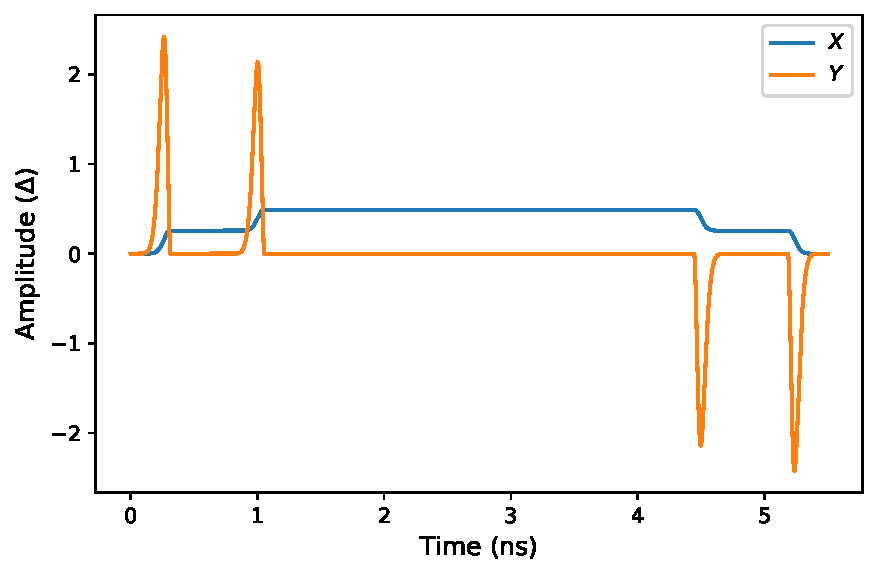
\includegraphics[width=0.8\columnwidth]{fig/fig_r2d_xy.pdf}
  \label{fig:r2d_xy}
  \caption{
    % Limitation of the proposed method for DRAG-2
    DRAG-2 pulse for $T=5.5~\text{ns}$.
    $t_r<\dfrac{2}{3}t_d$ degrades the gate performance and
    sharp edges arise in the $Y$ control.
  }
\end{figure}
In our proposed DRAG-2 design scheme,
using the echo method in the construction of the rising edge of $f(t)$ in \fref{fig:drag1} carries several difficulties.
First, it imposes us a minimum gate time limit as $ t_r>t_d/3 $,
$$
  T = 2t_d+t_r > 7/3t_d\quad\text{Our method.}
$$
If we could use a different method to construct $f(t)$ in \fref{fig:drag1}, this limit can be pushed to
$$
  T = 2t_d+t_r > 5/2t_d\quad\text{Theoretical limit.}
$$
The minimum gate duration degrades by $7\%$.
It has another problem of introducing edges into the $Y$ control pulse as illustrated in \fref{fig:r2d_xy}.
This is because if $t_r <2/3t_d$, $h(t)$ in \fref{fig:drag2} becomes short in duration.
Although designed as a DRAG-2 pulse, and inherently performs better than DRAG-1,
% \subsubsection{Simulation settings}
% \begin{figure}
%   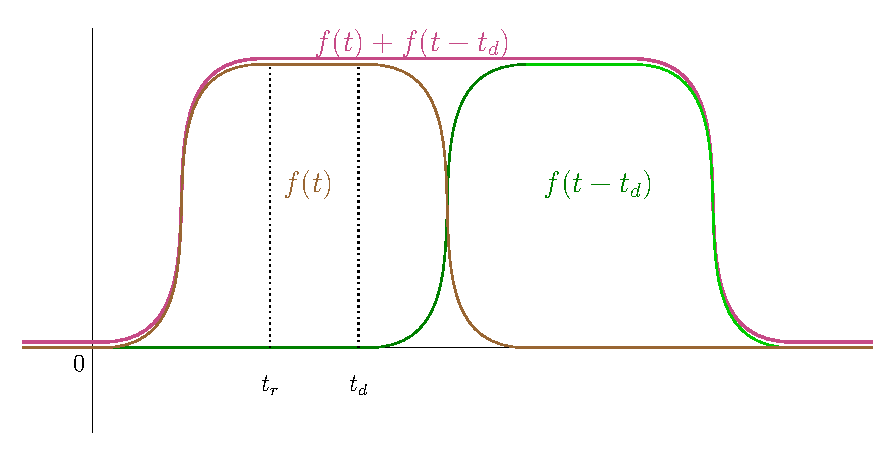
\includegraphics[scale=.3]{fig/fig_drag1.pdf}
% \end{figure}
% The
% is created with
% $ \Omega_1(t) = \Omega_0\sin^3(\pi t/T) $, which gives
% $$
%   \Omega(x) =
% $$
% The maximum value of which is

\subsubsection{Non-perturbative Validation of the $Y$-DRAG Correction}
Aside from the $X$ control pulse, we utilize the DRAG pulses \ref{eq:ydrag} and \ref{eq:zdrag}.
We demonstrate that the analytical expression for the $Y$ control pulse remains valid even in the non-perturbative
regime---a derivation that, to the best of our knowledge, has not been previously reported in the literature. To
illustrate this, we recalculate the system Hamiltonian without relying on perturbative assumptions. We introduce a
unitary frame transformation $V$, defined as:
\begin{equation}
  V = \exp\left[-i\lambda_2\dfrac{\Omegax}{2\Delta_2}\hat{\sigma}^y_{1,2}\right]
  = \cos(\phi) -i\hat{\sigma}^y_{1,2}\sin(\phi)
  \label{eq:first_frame_change}
\end{equation}
where $\phi = \lambda_2\dfrac{\Omegax}{2\Delta_2}$, and apply it to our qudit Hamiltonian in \eref{eq:Hrwa}.
The $\ket{1}\bra{2}$ component of the resulting Hamiltonian is
$$
  -\sin(2\phi)\dfrac{\delta(t)+\Delta}{2}+\cos(2\phi)\dfrac{\lambda \Omegax}{2}-i\dfrac{\lambda}{2}\left(\dfrac{\Omega_x^\prime(t)}{\Delta}+\Omega_y(t)\right).
$$
Substituting $\Omega_y$ as defined in \eref{eq:ydrag} demonstrates that this off-diagonal component is still effectively
suppressed. Consequently, we retain the standard DRAG correction  for the $Y$ control pulse.

\subsubsection{Hardware Constraint}
The proposed method utilizes a fast-rising flat-top pulse. We now evaluate the specifications such a pulse
demands from the control hardware. To determine whether an Arbitrary Waveform Generator (AWG) can physically synthesize
it, we must account for real-world hardware constraints---most notably the analog bandwidth limit and the slew rate limit.
For this analysis, we assess these requirements against the specifications of the following AWGs, which are widely
deployed in modern quantum computing architectures \cite{Keysight}:

\begin{itemize}
  \item Qblox QCM (1GSa/S, BW 400MHz)
  \item Zurich Instruments SHFQC+ (2 GSa/s, 800 MHz)
  \item Keysight M8195A (65 GSa/s, 25 GHz)
\end{itemize}

Furthermore, the target drive amplitude $\Omega_{x}$ and the physical AWG output voltage $V_{AWG}$ are not equivalent.
They are related by a system-specific calibration factor $c$:
$$\Omega_{x} = c V_{AWG}.$$
While the exact value of $c$ varies across different quantum processors, we assume $c = 50$ MHz/V for this
evaluation.
If the maximum AWG output is insufficient to reach the desired pulse amplitude under this conversion factor,
a room-temperature low-noise RF amplifier must be incorporated in the control line.

\subsubsection*{The Analog Bandwidth Limit}
By substituting $T=5.0~\text{ns}$ and $t_d=2.2~\text{ns}$ in $t_r+2t_d = T$, we have the estimate $t_r=0.6~\text{ns}$.
By applying the RC Low-Pass Rise Time Formula \cite{horowitz2015art}, the rise time limit is $\dfrac{0.35}{BW}$,
which is $0.43~\text{ns}$ for SHFQC+ and $0.86~\text{ns}$ for QCM.

% \noindent\textbf{Sampling Rate}\\
\subsubsection*{Sampling Rate}
An inadequate sampling rate at the rising edge will distort the synthesized pulse shape. If we assume a minimum of 5 to
6 samples is needed for accurate reproduction, the required rate is:
$$ \frac{1}{0.6 \text{ ns}} \times 5 = 8.3 \text{ GS/s} $$
While only the Keysight M8195A meets this threshold among the evaluated models, an AWG of this high grade is not strictly mandatory.

\noindent\textbf{The Slew Rate Limit}\\
Inspecting \fref{fig:r1d_comparison}, the amplitude can be estimated as $0.5\Delta$, which yields:
$$ \frac{0.5\Delta}{c} \approx 4.0~\text{V} $$
This indicates that the AWG alone, which generally outputs 1 to 2 V peak-to-peak, cannot generate the required voltage.
Therefore, a lab-grade external amplifier is required, though this remains a highly practical solution.

% \noindent\textbf{Summary}\\
% In summary, the proposed fast-rising flat-top pulse is realizable with the current hardware specs used in the control of quantum comupting.

\subsection{Riccati Engineering}
As for $\delta x_k$, we used the sum of two $\sin$ waves so that they the RHS of \eref{eq:riccati_variation} becomes $0$.
\begin{figure}[htpb]
  \centering
  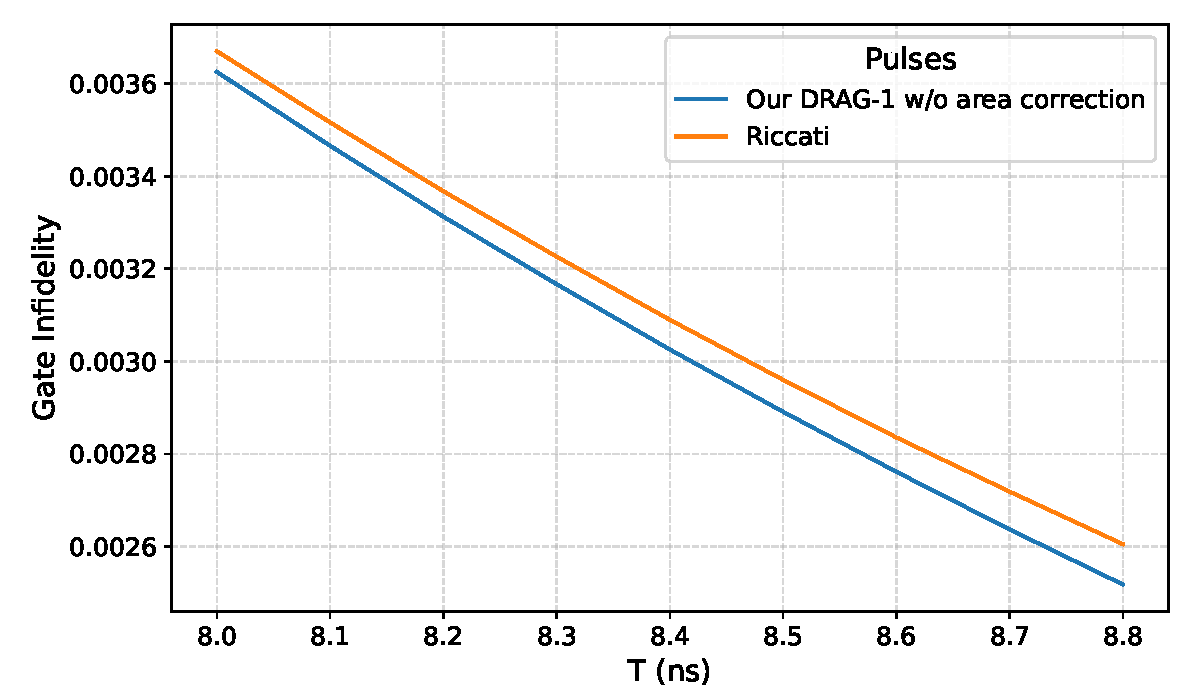
\includegraphics[width=0.8\columnwidth]{fig/fig_riccati.pdf}
  \label{fig:riccativsr1d}
  \caption{
    Our DRAG-1 pulses' performance when Riccati engineering applied.
    Riccati engineering had a little effect on gate infidelity.
  }
\end{figure}
Riccati engineering method generally failed to improve gate fidelity.
This is considered to be due to difficuly in numerical analysis.
% Further investigations
% They generally induces big error
% \subsubsection{Leakage}
% This gives us an insight that
% $\eps$

\subsection{CZ gate}
\subsubsection{Simulation}
% \epsilon
We set $N=1001$.
As in the previous research \cite{Ding2025,Martinis2014}, we simulate our designed pulses in the following fashion:
We design $\dfrac{\dd\theta}{\dd\tau}$ and then integrate to find $\theta$ in non-linear time frame.
We apply the time transformation to obtain $\theta(t)$.
We then simulate the time evolution as the two-level system described in \ref{subsec:leakage}
to find the leakage error.
We also simulate with the Hamiltonian in \eref{eq:hamiltonian_cz}
to find the phase accumulation of $\ket{00}$, $\ket{01}$ and $\ket{10}$.
We first simulate  with the normalized amplitude, changing this amplitude by an optimizer to find when the conditional
phase is close to $\pi$.
Also, Slepian pulse with $NW=2.9$ is used for reference.
% $$
%   \tilde{g}\rightarrow \tilde{\theta}\rightarrow x \rightarrow y
% $$
% Simulation conditions are
% We numerically solved the dynamics described in \ref{subsec:leakage},
% and then find $P_e$
\subsubsection{Anti-symmetric Chebyshev pulse}
\begin{figure}
  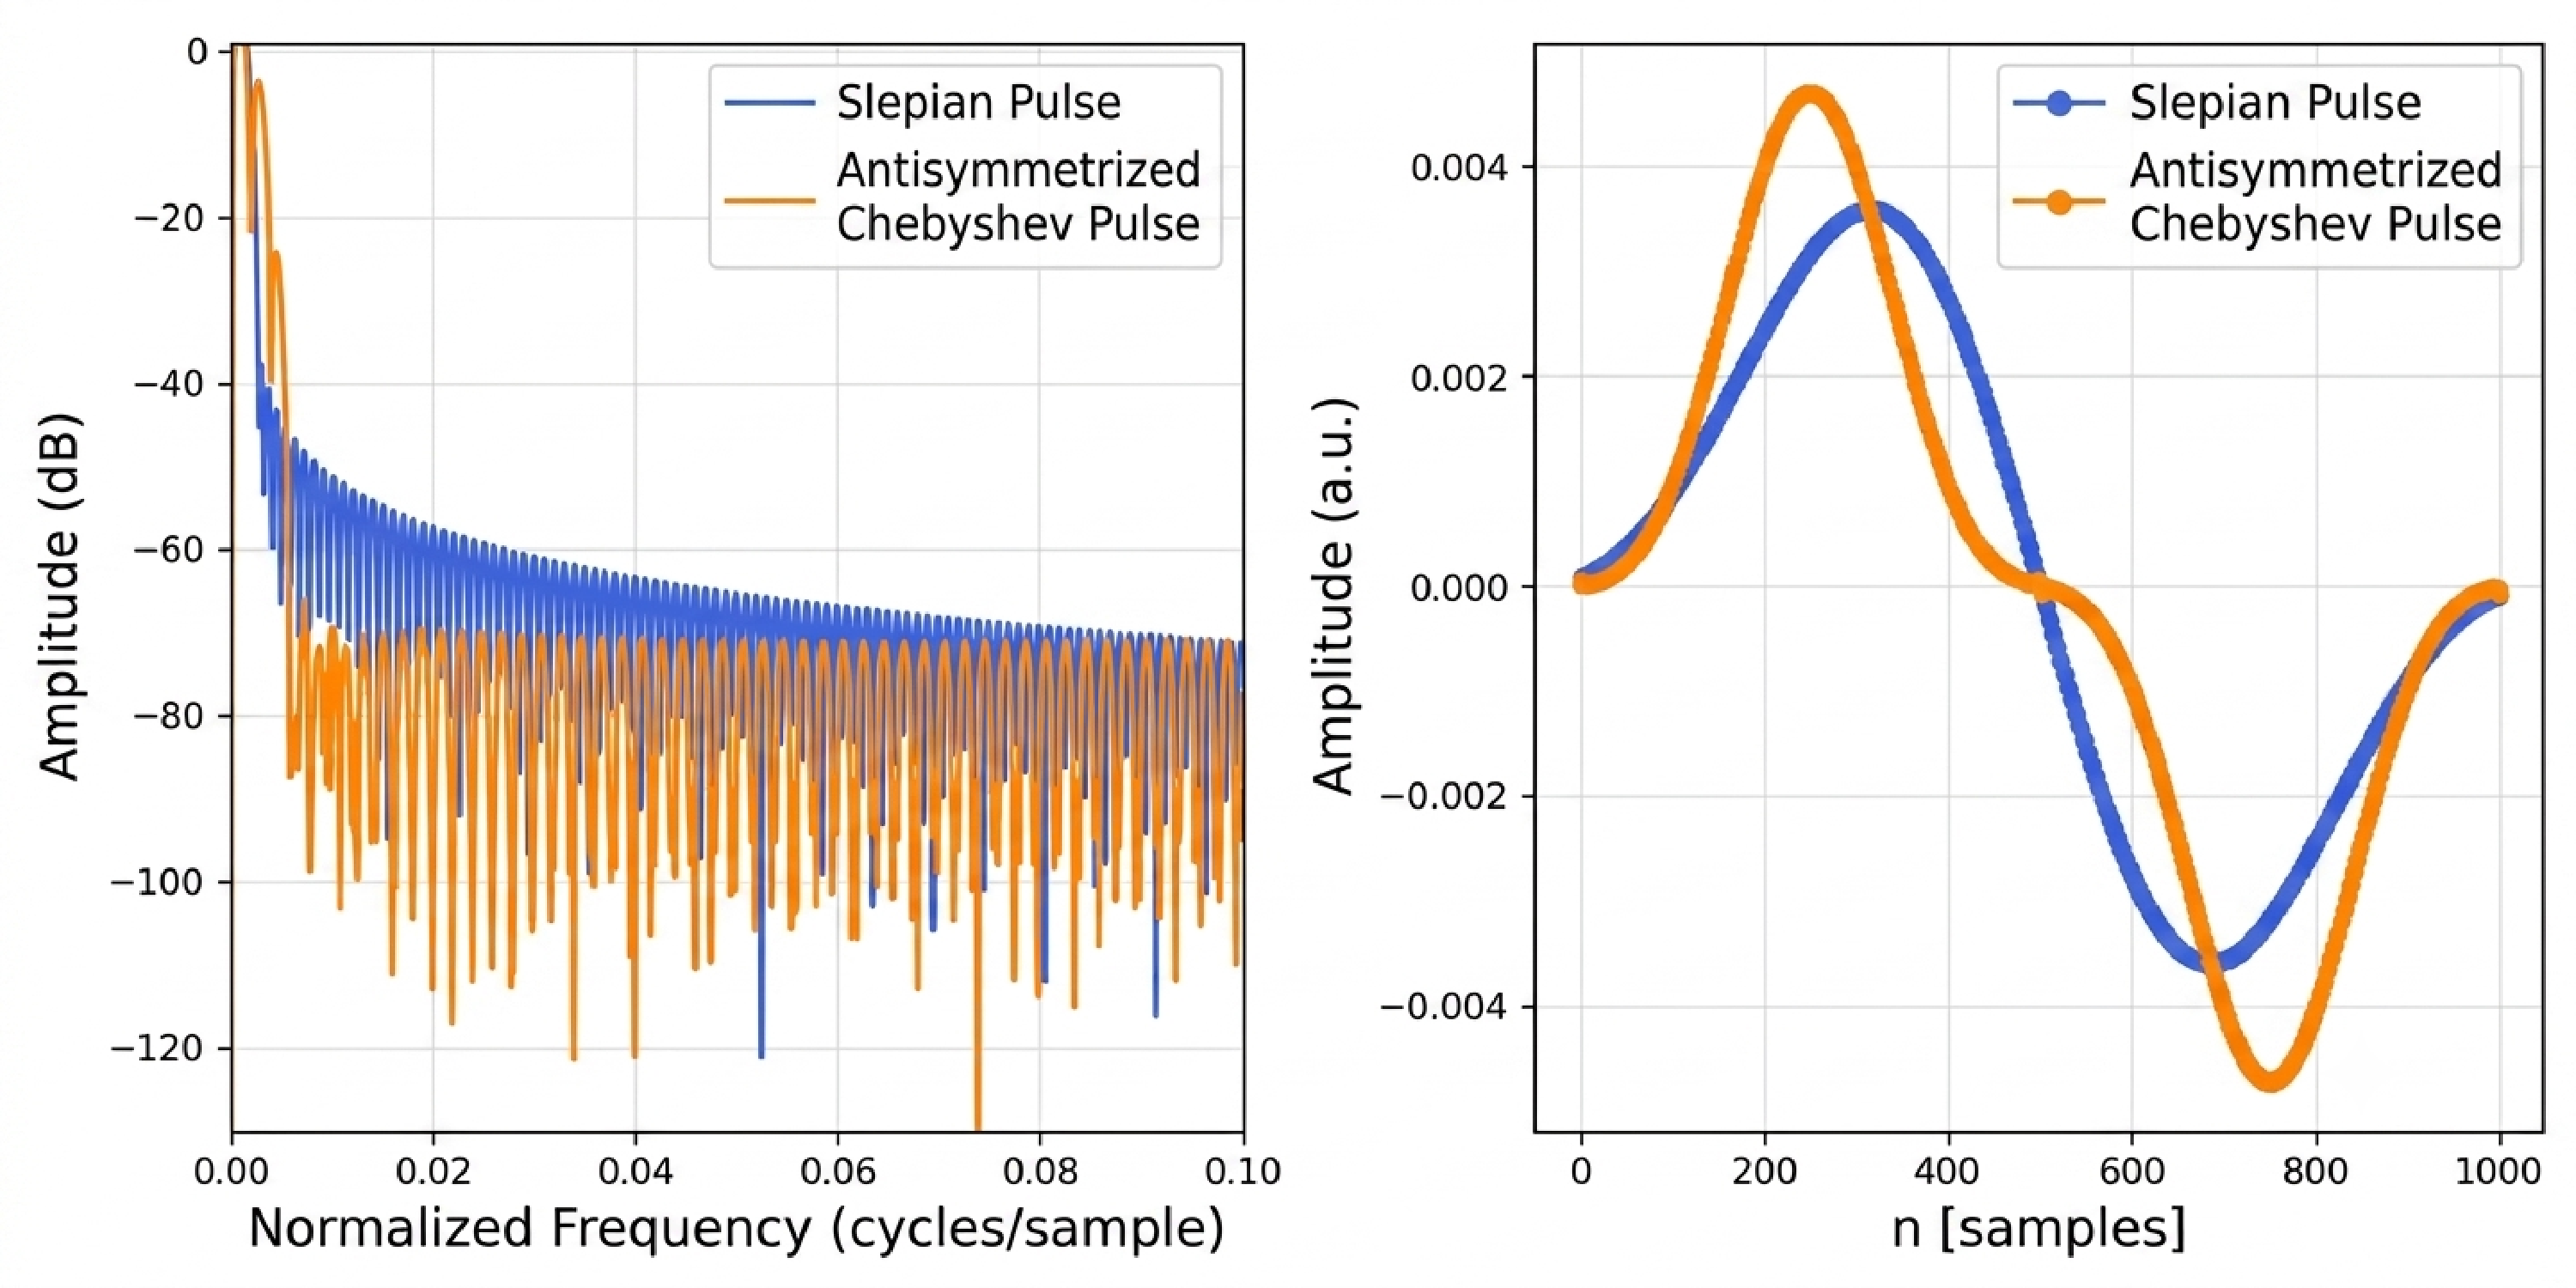
\includegraphics[scale=.3]{fig/fig_cheb_slep.pdf}
  \caption{
    The frequency domain (left) and the time domain (right) representation of Slepian and antisymmetrized Chebyshev
    pulses. The parameter $r$ is chosen so that sidelobe height is $40~\mathrm{dB}$ lower than the first slepian
    sidelobe height.
  }
  \label{fig:cheb_slep}
\end{figure}
Created with the parameter $r=0.000238$, this pulse is illustrated in \fref{fig:cheb_slep}
\subsubsection{Sidelobe-Aware Optimization}
\begin{figure}
  \centering
  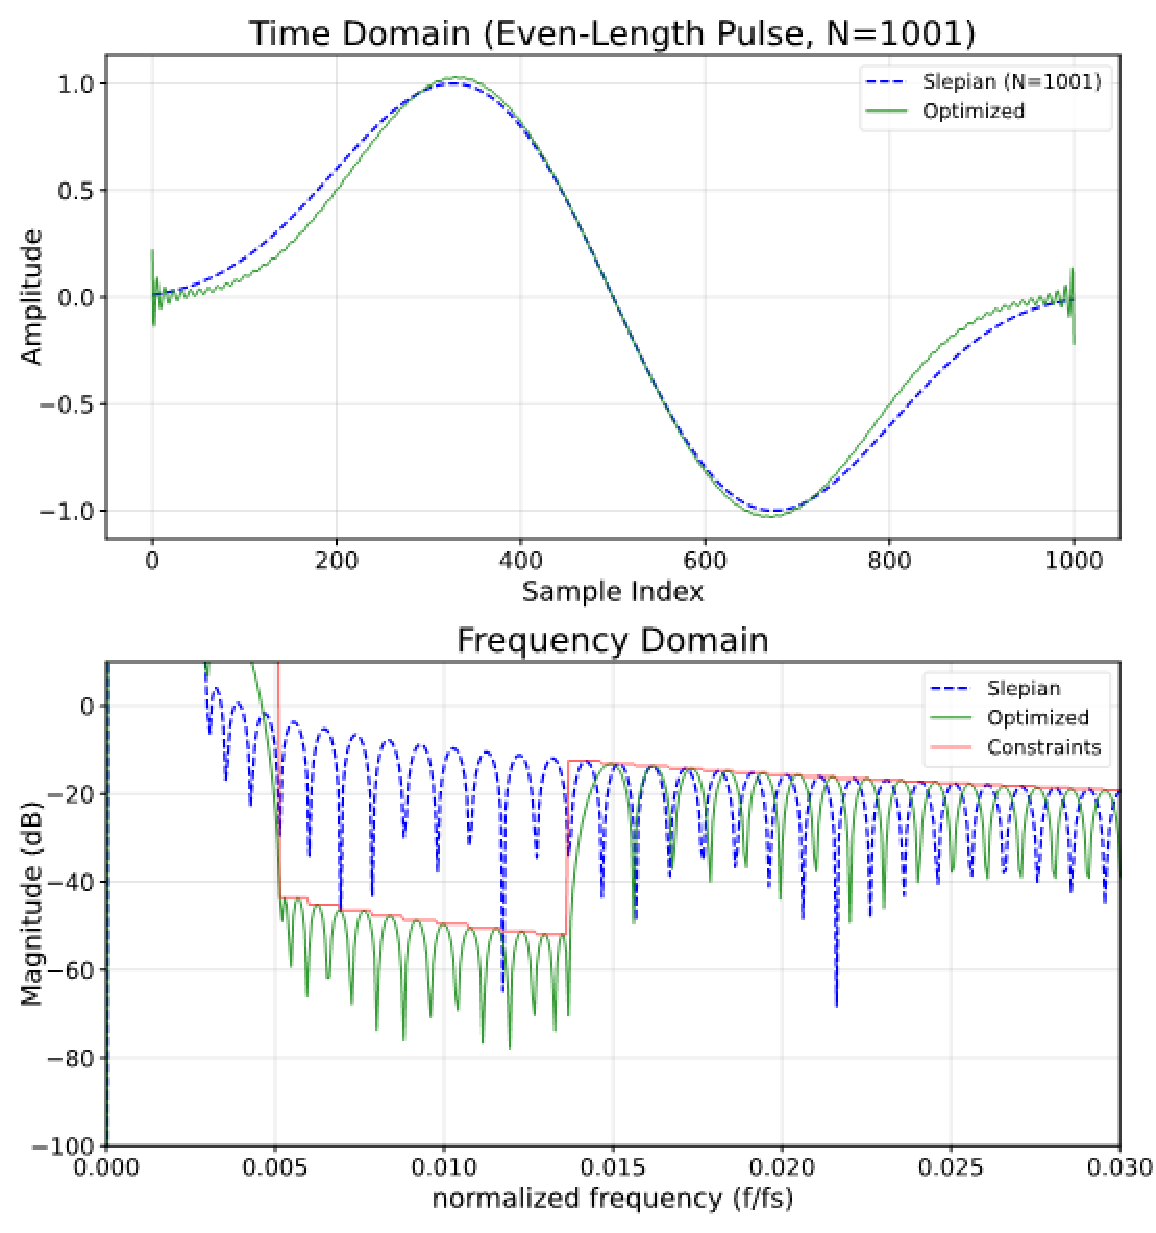
\includegraphics[scale=.5]{fig/fig_slep_opt.pdf}
  \caption{
    Slepian pulse and its optimized pulse.
    % The frequency domain (left) and the time domain (right) representation of Slepian and antisymmetrized Chebyshev
    % pulses. The parameter $r$ is chosen so that sidelobe height is $40~\mathrm{dB}$ lower than the first slepian
    % sidelobe height.
  }
  \label{fig:slep_opt}
\end{figure}
After the first four sidelobe, from $5$-th to $13$-th sidelobe heights are suppressed.
The pulse shape and its spectrum are illustrated in \fref{fig:slep_opt}.
\subsubsection{Slepian pulse with redefined maximization problem}
We set $W_1=2.9/1001$ and $W_2=8.8/1001$ to obtain a pulse with the corresponding redefined problem.
\subsubsection{Performance}
\begin{figure}[thbp]
  \centering
  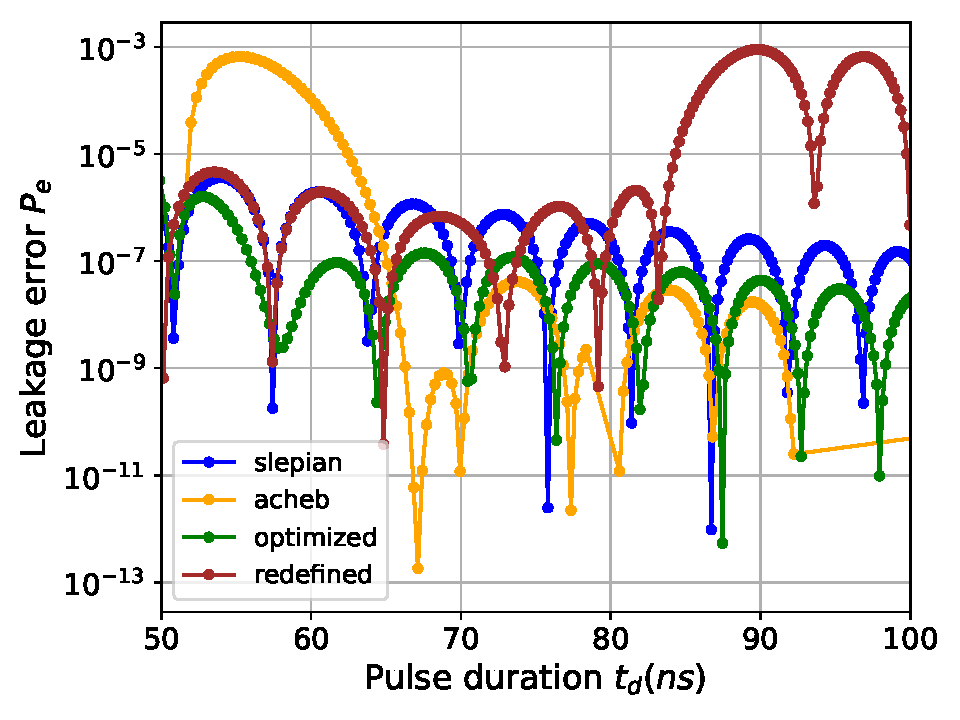
\includegraphics[width=.5\textwidth]{fig/fig_redefined.pdf}
  \caption{Leakage error of four pulses, Slepian (slepian), Anti-symmetric Chebyshev (acheb), Sidelobe-aware
    optimization (optimized), and the pulse optimized by redefining the original eigenvalue problem (redefined)}
  \label{fig:performance_cz}
\end{figure}
As illustrated in \fref{fig:performance_cz}, in overall, the optimized slepian pulse performed the best.
The anti-symmetric Chebyshev pulse performed really well at around $T=70~\text{ns}$ with suppressing leakage level by an
order of two.
The result of the Slepian pulse with the redefined problem is aligned with our expectations, larger leakage error at
unwanted gate duration times.
\subsubsection{Minimum Gate time}
\begin{figure}
  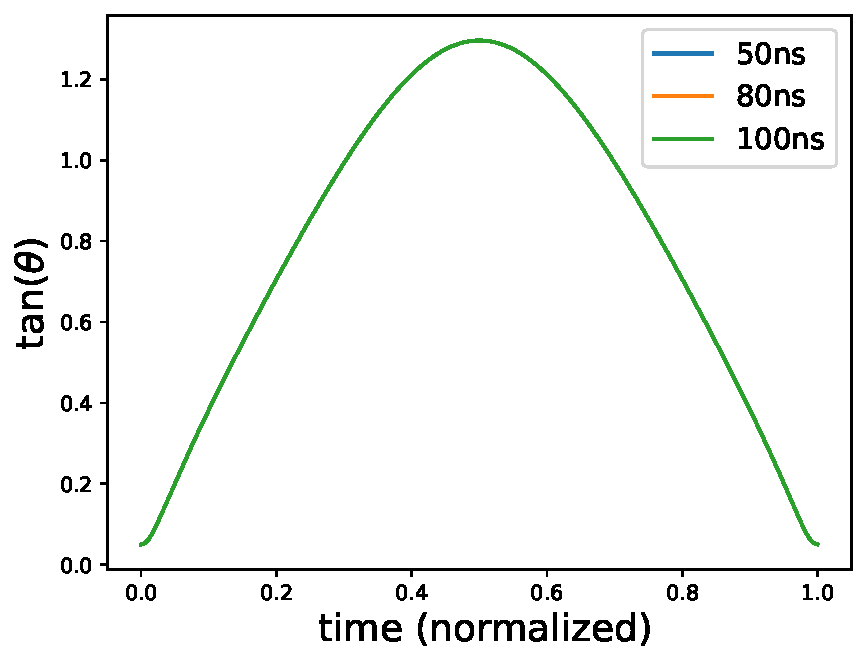
\includegraphics[scale=.5]{fig/fig_tan_5080100.pdf}
  \centering
  \caption{The relation between $T_d$ and $\tan(\theta)$ for the Slepian pulse with $T=50,80,100 $. The three
    graphs are overlapping each other due to almost the same $A(\tau_d)$.}
  \label{fig:amplitude}
\end{figure}
Once the pulse shape ${g}$ determined,
its integration ${\theta}$ is decided up to the amplitude factor $A(\tau_d)$, $(0\leq A(\tau_d)\leq1)$
$$
  {\theta} = {\theta}^n(\tau/\tau_d)A(\tau_d),
$$
where ${\theta}^n$ is the normalized ${\theta}$ that reaches $\epsilon(t_{mid})=0$ during avoided crossing.
\begin{align*}
  t(\tau) & = \int_0^\tau \sin {\theta}(\tau') \, \dd\tau'                                            \\
          & = \tau_d \int_0^{\tau/\tau_d}\,\sin \left[A(\tau_d) {\theta}^n(\tau') \right]\, \dd\tau'. \\
\end{align*}
% During this flux trajectory, the states $\vert{}00\rangle$, $\vert{}01\rangle$, and $\vert{}10\rangle$ remain largely
% isolated from any crossings. Therefore, the phases they accumulate are purely their standard, uncoupled dynamical
% phases:
% $\phi_{00} = \phi_{00}^{\text{uncoupled}}$$\phi_{01} = \phi_{01}^{\text{uncoupled}}$$\phi_{10} = \phi_{10}^{\text{uncoupled}}$
Therefore, gate duration in the lab frame is $t_d = \tau_d \int_0^1 \sin \left[A(\tau_d) {\theta}^n(\tau') \right]\, \dd\tau'$.
$t_d$ is decided upon the amplitude $A(\tau_d)$ and the initial pulse shape.
As you see in \fref{fig:amplitude},  $A(\tau_d)$ does not change over different $\tau_d$.
Hence the gate durations in $t$ and $\tau$ are proportionate.

% There are two types of phases: Berry phases and dynamical phases.
% Since the trajectory that the instantaneous $\ket{11}$ traces through the operation is a 1D path,
% thus enclosing zero area, it produces zero Berry phase.
% In formula,
% \begin{equation}
%   \phi = \int \Delta E \,\dd t = -\int \frac{\Delta}{2} \tan \frac{\theta(t)}{2} \, \dd t
% \end{equation}
%
% Since $\tan(\theta/2) = \dfrac{\tan(\theta)}{1+\sqrt{1+\tan(\theta)^2}}$
%
% % As you see in the graph of $\epsilon(t)$
% Since $0\leq\tan\dfrac{\theta(t)}{2}\leq 1$, the gate duration $T$ satisfies $T\geq \dfrac{2\pi}{\Delta}.$

% is connected through
%
% Required slew rate of DAC is


% \subsubsection{Combination of two pulses}
% Interestingly enough, their arguments are almost equal defying the possibility of mixing them together to gain a pulse
% with lower leakage.
% \subsubsection{Robustness against gate time}
% The reason behind the fact that the Slepian pulse has been used for so long days is its robustness against gate
% duration.
